\documentclass[presentation]{beamer}
\usepackage[utf8]{inputenc}
\usepackage[T1]{fontenc}
\usepackage{fixltx2e}
\usepackage{graphicx}
\usepackage{longtable}
\usepackage{float}
\usepackage{wrapfig}
\usepackage{rotating}
\usepackage[normalem]{ulem}
\usepackage{amsmath}
\usepackage{textcomp}
\usepackage{marvosym}
\usepackage[integrals]{wasysym}
\usepackage{amssymb}
\usepackage{hyperref}
\tolerance=1000
\usepackage{minted}
\usepackage{amsmath}
\usepackage{tikz}
\usepgflibrary{shapes.geometric}
\usetikzlibrary{calc}
\usetikzlibrary{positioning}
\usetikzlibrary{intersections,decorations.pathreplacing,shapes,arrows}
\usetikzlibrary{plotmarks}
\usepackage{amsmath,amssymb}
\usepackage{mathtools}
\DeclareMathOperator{\tr}{tr}
\usepackage{pgfplots}
\institute{Departments of Computing and Mathematics, Imperial College London}
\renewcommand{\vec}{\mathbf}
\usepackage{hyperref}
\hypersetup{breaklinks=true,
  urlcolor=blue,
colorlinks=true}
\newcommand{\arxivlink}[2]{%
  \href{http://www.arxiv.org/abs/#1}%
  {{\small\texttt{arxiv\,#1\,[#2]}}}%
}
\usetheme{IC}

\author{Lawrence Mitchell}
\date{2 September 2015}
\title{Firedrake: automating the finite element method by composing
  abstractions}

\usepackage[backend=biber,
            doi=true,
            url=false,
            isbn=false,
            maxbibnames=3,
            style=authoryear,
            firstinits=true]{biblatex}
\setlength{\bibitemsep}{0pt}
\DeclareFieldFormat{pages}{#1}
\DeclareFieldFormat[article,periodical]{volume}{\textbf{#1}}
\bibliography{references}
\begin{document}

\maketitle

\begin{frame}
  \frametitle{Introduction}
  \begin{center}
    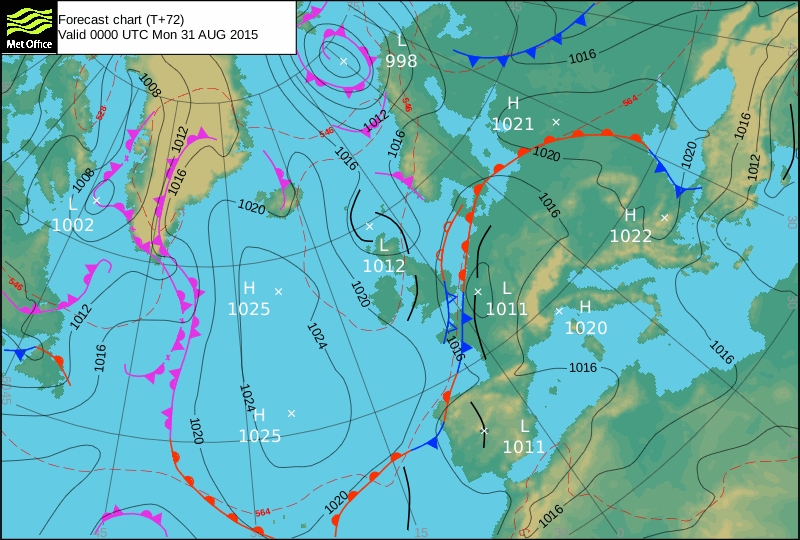
\includegraphics[width=\textwidth]{09-03-ParCo-firedrake-overview.figures/pressure}
  \end{center}
\end{frame}

\begin{frame}
  \frametitle{Simulation}
  \begin{enumerate}[<+->]
  \item Write down the equations.  Find $u$ s.t.\ $F(u) = 0$.
  \item Discretise.  Find $u_h$ s.t.\ $F_h(u_h) = 0$.
  \item Implement on computer.
  \item \ldots{}
  \item \ldots{}add all the bits that your discretisation didn't capture to
    get a decent answer.
  \end{enumerate}

  \begin{block}<+->{Problem}
    All these steps are hard, and require differing expertise
  \end{block}
\end{frame}

\begin{frame}
  \frametitle{In an ideal world}
  
  \begin{itemize}[<+->]
  \item Implementing discrete system would not require huge expertise
    in high performance computing.
  \item Providing the high performance implementation would not
    require huge expertise in the particular numerical methods.
  \end{itemize}

  \begin{block}<+->{Problem}
    I don't think this division can be sharp.  But, what can we do?
  \end{block}
\end{frame}


\begin{frame}
  \frametitle{Common themes in mesh-based PDE solvers}
  \begin{itemize}
  \item Local operators
  \item Iteration over mesh entities
  \item gathers and scatters from global to local data
  \end{itemize}

  \begin{block}<+->{Local operators}
    Have some (local) stencil, logically operate on contiguous local
    data.  Specified by PDE and choice of numerical method
  \end{block}
  \begin{block}<+->{Iteration} Evaluate local operators on (subsets
    of) mesh entities.  Pack (sparse) global data to (dense) local
    data.
  \end{block}
\end{frame}

\begin{frame}[fragile]
  \frametitle{Local operators: FE discretisations}
  \begin{itemize}
  \item Choice of function spaces, plus variational formulation is a
    \emph{declarative} specification of local operator.
  \item \ldots{}plus choice of quadrature, ...
  \end{itemize}
  \begin{onlyenv}<1>
\begin{minted}[fontsize=\scriptsize]{python}
# u the input fields (e.g. current guess)
def form_residual(u):
    u_l <- u # global to ghosted
    for each element in mesh:
        u_e <- u_l[element] # gather through element map
        for each qp in element:
            basis_fns <- eval_basis_funs(qp)
            J <- compute_geometry(element, qp)
            f_qp <- user_evaluation(qp, basis_fns, u_e)
            # insert into element residual
            f_e <- transform_to_physical(f_qp, J)
        f_l <- f_e # scatter through element map
    f <- f_l # ghosted to global
\end{minted}
  \end{onlyenv}
  \begin{block}<2->{Library division line}
\begin{minted}[fontsize=\scriptsize]{python}
            f_qp <- user_evaluation(qp, basis_fns, u_e)
\end{minted}    
    \begin{enumerate}
    \item User controls all mesh iteration.
    \item User provides element kernel.
    \item User only provides quad-point kernel.
    \end{enumerate}
  \end{block}
\end{frame}

\begin{frame}[t]
  \frametitle{Tradeoffs}
  \begin{block}<1-2 | only@1-2>{Type I}
    \begin{itemize}
    \item Library provides iteration constructs
    \item user provides \emph{full element loop}
    \end{itemize}
  \end{block}
  \begin{itemize}[<1-2 | only@2>]
  \item Full flexibility, can fuse across elements, cancel geometric
    transformations, etc...
  \item Can apply vectorization (and compiler may do good job,
    everything in one compilation unit)
  \item but, code commits to an implementation
  \end{itemize}
  \begin{block}<only@3-4>{Type II}
    \begin{itemize}
    \item Library iterates over mesh entities
    \item user provides \emph{element kernel}
    \end{itemize}
  \end{block}
  \begin{itemize}[<only@4>]
  \item code doesn't commit to an inter-element implementation
  \item can vectorize inside elements, difficult across elements (if a
    header-based library, maybe compiler will do it)
  \end{itemize}
  \begin{block}<only@5-6>{Type III}
    \begin{itemize}
    \item Library iterates over elements and quad points
    \item user provides \emph{pointwise function}
    \end{itemize}
  \end{block}
  \begin{itemize}[<only@6>]
  \item code doesn't commit to iteration at all
  \item but, can't exploit wider structure without provision of
    additional info
  \item unlikely to vectorize across quad points (again, header-based
    libraries might save you)
  \end{itemize}

  \begin{block}<+(6)->{Lemma}
    Compiler writers are not magicians.  If you, with your domain
    knowledge, are unable to provide an optimal implementation, it's
    unlikely that your compiler will.
  \end{block}
  \begin{block}<+(6)->{Corollary}
    Endeavour to provide ``easy to optimize'' code.
  \end{block}
\end{frame}

\begin{frame}
  \frametitle{More complex transformations}
  \begin{itemize}[<+->]
  \item On top of inlining, we might want to do other things
  \item e.g.\ locally invert element matrices (static condensation)
  \item Reorder data and fuse across elements
  \item Reorder data and split within elements (e.g.\ for GPUs)
  \item The best optimisations are \emph{order} and \emph{hardware}
    dependent.  But wouldn't it be nice if we still had \emph{one}
    source.
  \end{itemize}
  \begin{block}<+->{Numerical ``meta-computing''}
    Many of these transformations are \emph{mechanical} if only we
    could express what we wanted.
  \end{block}
\end{frame}
\begin{frame}
  \frametitle{Firedrake}
  \begin{itemize}
  \item User interface for FE problems through
    UFL \parencite{Alnaes:2014}
  \item Mesh iteration via PyOP2 \parencite{Rathgeber:2012}
  \item \arxivlink{1501.01809}{cs.MS} 
  \end{itemize}
  \begin{block}{Design choices}
    \begin{itemize}[<+->]
    \item Try not to commit model developer to a low-level
      implementation.
    \item Code generation from high-level symbolic descriptions where
      possible.
    \item ``User'' provides full element kernel (automated compilation
      from UFL)
    \item Mesh library provides abstract iteration construct (exposed
      to user)
    \end{itemize}
  \end{block}
\end{frame}

\begin{frame}{Example}
\begin{block}{Phase separation}
{\scriptsize \begin{equation*}
\begin{aligned}
F[\phi(x, t)] &= \int \overbrace{\alpha \phi^2 + \beta \phi^4 + \epsilon}^{\mathclap{\text{Landau potential}}} + \underbrace{\frac{\gamma}{2} |\nabla\phi|^2}_{\mathclap{\text{interface penalty}}}\,\mathrm{d}x\\
\mu = \frac{\delta F}{\delta \phi} &= 2\alpha\phi + 4\beta\phi^3 - \gamma\nabla^2\phi\\
\frac{\partial \phi}{\partial t} &= \nabla \cdot D(\phi) \nabla \mu
\end{aligned}
\end{equation*}
}
Find $\phi, \mu \in V \times V \subset H^1 \times H^1$ such that
{\scriptsize \begin{equation*}
\begin{aligned}
\langle \phi^{n+1} - \phi^n, q \rangle + \Delta t D \langle \nabla ((1 - \theta)\mu^{n} + \theta \mu^{n+1}), \nabla q \rangle &= 0 \quad \forall\, q \in V\\
\langle \mu - \partial_\phi f, v \rangle - \gamma \langle \nabla \phi, \nabla v \rangle &= 0 \quad \forall\, v \in V\\
n\cdot\nabla \phi = n\cdot\nabla \mu &= 0 \quad\text{on $\partial\Omega$}
\end{aligned}
\end{equation*}
}
\end{block}
\end{frame}
\begin{frame}[fragile]{Code}
 \begin{minted}[fontsize=\scriptsize]{python}
mesh = Mesh("some_domain.msh")
V = FunctionSpace(mesh, "CG", 1)
W = V*V
gamma = Constant(0.005)
D = Constant(10)
q, v = TestFunctions(W)
u = Function(W)
u0 = Function(W)
phi, mu = split(u)
phi0, mu0 = split(u0)
phi = variable(phi)
f = 10*(phi**2 - 1)**2
dfdphi = diff(f, phi)
theta = 0.5
mu_theta = (1-theta)*mu0 + theta*mu
dt = 5e-6
F = ((phi - phi0)*q + dt*D*dot(grad(mu_theta), grad(q)) +
     (mu - dfdphi)*v - gamma*dot(grad(phi), grad(v)))*dx
for _ in range(200):
    u0.assign(u)
    solve(F == 0, u)
\end{minted}
\end{frame}
\begin{frame}
  \frametitle{Why symbolic?}
  \begin{itemize}
  \item FE lends itself to DSLs, hence the success of the FEniCS
    project\footcite{Logg:2012}
  \item More than just sugar!
  \item Single source can be transformed to give different
    implementations.
  \item I think this is increasingly important to allow a single
    codebase to perform well on varied hardware: e.g.\ matrix-free as
    opposed to assembled operators.
  \end{itemize}
\end{frame}
\begin{frame}
  \frametitle{Abstract iteration}
  \begin{itemize}[<+->]
  \item Express the what, not the how.
  \item Iteration library sees ``tasks'' with data dependencies.
    Doesn't \emph{care} about application control flow.
  \item Things like loop tiling can live in the library
  \item Need to iterate over some new entity?  Just build the data
    structure: no need for special casing.
  \end{itemize}
\end{frame}

\begin{frame}[fragile]
  \frametitle{Example}
  Spin over cells, write max cell value into vertices (part of a slope
  limiter).

\begin{minted}[fontsize=\scriptsize]{python}
max_field = Function(P1)
centroids = Function(P0DG)
...
par_loop("""
for (int i=0; i<qmax.dofs; i++) {
    qmax[i][0] = fmax(qmax[i][0], centroids[0][0]);
}
""",
   dx,
   {'qmax': (max_field, RW),
    'centroids': (centroids, READ)})
\end{minted}
\end{frame}
\begin{frame}[fragile]
  \frametitle{Good Things\footnotemark[1]}
  \footnotetext[1]{with apologies to Sellar \& Yeatman}
  \begin{itemize}
  \item Expressing purely variational problems is easy (and natural?)
  \item ``Symbolic'' (lazily evaluated) mesh iteration allows for mesh
    tiling
  \item Writing C kernels for non-variational things is not \emph{too}
    taxing (still get all the other bits for free).
  \item Code generation keeps codebase \emph{small} (maintainability).
  \item Can explore code optimisations that may, for complicated
    problems, be difficult to do by
    hand \parencite{Olgaard:2010,Luporini:2015}.  Observe 70\% FP peak
    for element tensor assembly on P3 tets.
  \end{itemize}
\end{frame}

\begin{frame}
  \frametitle{Bad Things}
  \begin{itemize}
  \item DSLs are not all gravy: things that don't fit need abstraction
    design, plus implementation.  Can't hack something together.
  \item Runtime code generation can be a pain on HPC systems.
  \item Overhead of runtime symbolic manipulations \emph{hurts} strong
    scaling.
  \end{itemize}
  \begin{uncoverenv}<2->
    \begin{center}
      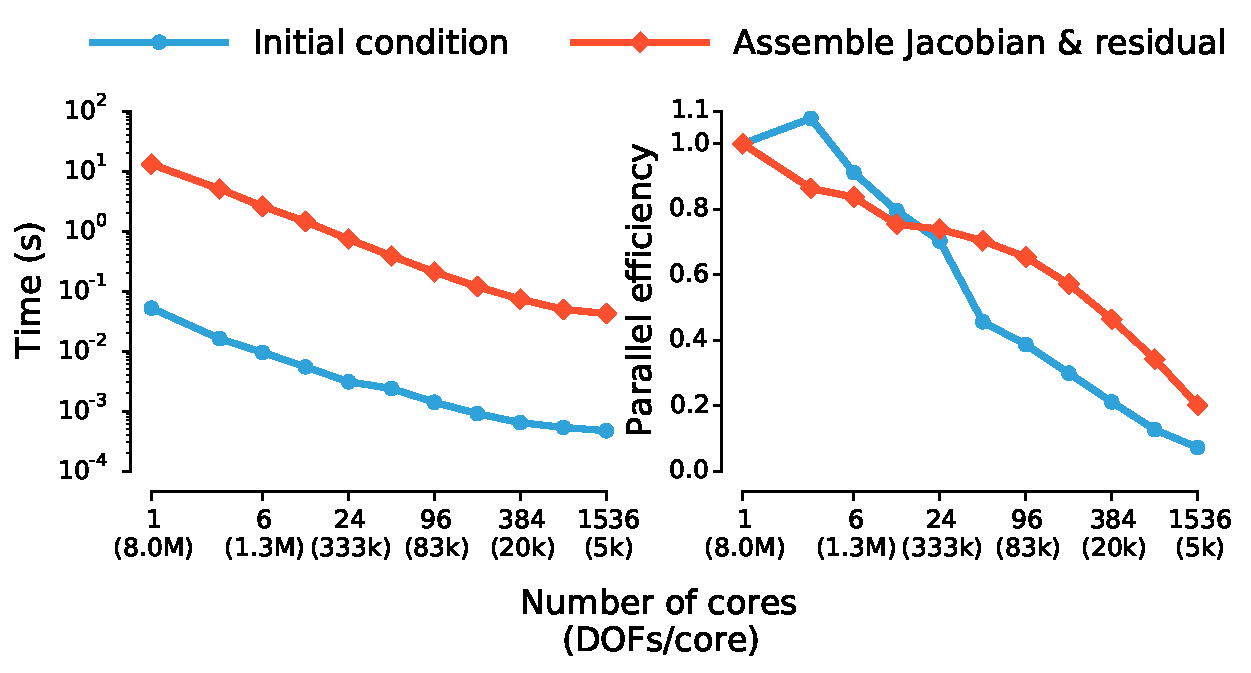
\includegraphics[height=0.75\textheight]{09-03-ParCo-firedrake-overview.figures/strong-scaling}
    \end{center}
  \end{uncoverenv}
\end{frame}

\begin{frame}
  \frametitle{Conclusions}
  \begin{itemize}
  \item I think DSLs are a fine way to provide an interface for PDE
    solvers
  \item \ldots\ but there's no free lunch.
  \item A lot of the design decisions that you might take when
    designing a DSL-based language carry over to more general purpose
    libraries.
  \item Aim to build libraries such that user
    writes data parallel code.
  \item Try not to tie application code to a ``low-level'' implementation.
  \end{itemize}
\end{frame}

\begin{frame}
  \frametitle{Thanks}
  \begin{block}{The Firedrake team}
    \href{http://firedrakeproject.org/team.html}{firedrakeproject.org/team.html}
  \end{block}
  \begin{block}{Funding}
    \begin{itemize}
    \item EPSRC: EP/L000407/1, EP/K008730/1, EP/I00677X/1
    \item NERC: NE/K008951/1, NE/K006789/1, NE/G523512/1
    \item The Grantham Institute for climate change
    \end{itemize}
  \end{block}
  \begin{center}
    \href{http://www.firedrakeproject.org}{www.firedrakeproject.org}\\
    \href{http://github.com/firedrakeproject/firedrake}{github.com/firedrakeproject/firedrake}
  \end{center}
\end{frame}

\begin{frame}
  \frametitle{References}
  \renewcommand*{\bibfont}{\footnotesize}
  \printbibliography
\end{frame}
\end{document}
